% Created 2021-04-12 Mon 13:10
% Intended LaTeX compiler: pdflatex

\documentclass[english]{article}
\usepackage[T1, T2A]{fontenc}
\usepackage[lutf8]{luainputenc}
\usepackage[english, russian]{babel}
\usepackage{minted}
\usepackage{graphicx}
\usepackage{longtable}
\usepackage{hyperref}
\usepackage{xcolor}
\usepackage{natbib}
\usepackage{amssymb}
\usepackage{stmaryrd}
\usepackage{amsmath}
\usepackage{caption}
\usepackage{mathtools}
\usepackage{amsthm}
\usepackage{tikz}
\usepackage{grffile}
\usepackage{extarrows}
\usepackage{wrapfig}
\usepackage{algorithm}
\usepackage{algorithmic}
\usepackage{lipsum}
\usepackage{rotating}
\usepackage{placeins}
\usepackage[normalem]{ulem}
\usepackage{amsmath}
\usepackage{textcomp}
\usepackage{capt-of}

\usepackage{geometry}
\geometry{a4paper,left=2.5cm,top=2cm,right=2.5cm,bottom=2cm,marginparsep=7pt, marginparwidth=.6in}
 \usepackage{hyperref}
 \hypersetup{
     colorlinks=true,
     linkcolor=blue,
     filecolor=orange,
     citecolor=black,      
     urlcolor=cyan,
     }

\usetikzlibrary{decorations.markings}
\usetikzlibrary{cd}
\usetikzlibrary{patterns}
\usetikzlibrary{automata, arrows}

\newcommand\addtag{\refstepcounter{equation}\tag{\theequation}}
\newcommand{\eqrefoffset}[1]{\addtocounter{equation}{-#1}(\arabic{equation}\addtocounter{equation}{#1})}
\newcommand{\llb}{\llbracket}
\newcommand{\rrb}{\rrbracket}


\newcommand{\R}{\mathbb{R}}
\renewcommand{\C}{\mathbb{C}}
\newcommand{\N}{\mathbb{N}}
\newcommand{\A}{\mathfrak{A}}
\newcommand{\B}{\mathfrak{B}}
\newcommand{\rank}{\mathop{\rm rank}\nolimits}
\newcommand{\const}{\var{const}}
\newcommand{\grad}{\mathop{\rm grad}\nolimits}

\newcommand{\todo}{{\color{red}\fbox{\text{Доделать}}}}
\newcommand{\fixme}{{\color{red}\fbox{\text{Исправить}}}}

\newcounter{propertycnt}
\setcounter{propertycnt}{1}
\newcommand{\beginproperty}{\setcounter{propertycnt}{1}}

\theoremstyle{plain}
\newtheorem{propertyinner}{Свойство}
\newenvironment{property}{
  \renewcommand\thepropertyinner{\arabic{propertycnt}}
  \propertyinner
}{\endpropertyinner\stepcounter{propertycnt}}
\newtheorem{axiom}{Аксиома}
\newtheorem{lemma}{Лемма}
\newtheorem{manuallemmainner}{Лемма}
\newenvironment{manuallemma}[1]{%
  \renewcommand\themanuallemmainner{#1}%
  \manuallemmainner
}{\endmanuallemmainner}

\theoremstyle{remark}
\newtheorem*{remark}{Примечание}
\newtheorem*{solution}{Решение}
\newtheorem{corollary}{Следствие}[theorem]
\newtheorem*{examp}{Пример}
\newtheorem*{observation}{Наблюдение}

\theoremstyle{definition}
\newtheorem{task}{Задача}
\newtheorem{theorem}{Теорема}[section]
\newtheorem*{definition}{Определение}
\newtheorem*{symb}{Обозначение}
\newtheorem{manualtheoreminner}{Теорема}
\newenvironment{manualtheorem}[1]{%
  \renewcommand\themanualtheoreminner{#1}%
  \manualtheoreminner
}{\endmanualtheoreminner}
\captionsetup{justification=centering,margin=2cm}
\newenvironment{colored}[1]{\color{#1}}{}

\tikzset{->-/.style={decoration={
  markings,
  mark=at position .5 with {\arrow{>}}},postaction={decorate}}}
\makeatletter
\newcommand*{\relrelbarsep}{.386ex}
\newcommand*{\relrelbar}{%
  \mathrel{%
    \mathpalette\@relrelbar\relrelbarsep
  }%
}
\newcommand*{\@relrelbar}[2]{%
  \raise#2\hbox to 0pt{$\m@th#1\relbar$\hss}%
  \lower#2\hbox{$\m@th#1\relbar$}%
}
\providecommand*{\rightrightarrowsfill@}{%
  \arrowfill@\relrelbar\relrelbar\rightrightarrows
}
\providecommand*{\leftleftarrowsfill@}{%
  \arrowfill@\leftleftarrows\relrelbar\relrelbar
}
\providecommand*{\xrightrightarrows}[2][]{%
  \ext@arrow 0359\rightrightarrowsfill@{#1}{#2}%
}
\providecommand*{\xleftleftarrows}[2][]{%
  \ext@arrow 3095\leftleftarrowsfill@{#1}{#2}%
}
\makeatother

\newenvironment{rualgo}[1][]
  {\begin{algorithm}[#1]
     \selectlanguage{russian}%
     \floatname{algorithm}{Алгоритм}%
     \renewcommand{\algorithmicif}{{\color{red}\textbf{если}}}%
     \renewcommand{\algorithmicthen}{{\color{red}\textbf{тогда}}}%
     \renewcommand{\algorithmicelse}{{\color{red}\textbf{иначе}}}%
     \renewcommand{\algorithmicend}{{\color{red}\textbf{конец}}}%
     \renewcommand{\algorithmicfor}{{\color{red}\textbf{для}}}%
     \renewcommand{\algorithmicto}{{\color{red}\textbf{до}}}%
     \renewcommand{\algorithmicdo}{{\color{red}\textbf{делать}}}%
     \renewcommand{\algorithmicwhile}{{\color{red}\textbf{пока}}}%
     \renewcommand{\algorithmicrepeat}{{\color{red}\textbf{повторять}}}%
     \renewcommand{\algorithmicuntil}{{\color{red}\textbf{до тех пор пока}}}%
     \renewcommand{\algorithmicloop}{{\color{red}\textbf{повторять}}}%
     \renewcommand{\algorithmicnot}{{\color{blue}\textbf{не}}}%
     \renewcommand{\algorithmicand}{{\color{blue}\textbf{и}}}%
     \renewcommand{\algorithmicor}{{\color{blue}\textbf{или}}}%
     \renewcommand{\algorithmicrequire}{{\color{blue}\textbf{Предусловие}}}%
     \renewcommand{\algorithmicrensure}{{\color{blue}\textbf{Постусловие}}}%
     \renewcommand{\algorithmicrtrue}{{\color{blue}\textbf{истинна}}}%
     \renewcommand{\algorithmicrfalse}{{\color{blue}\textbf{ложь}}}%
     % Set other language requirements
  }
  {\end{algorithm}}
\author{Ilya Yaroshevskiy}
\date{\today}
\title{Лекция 9}
\hypersetup{
 pdfauthor={Ilya Yaroshevskiy},
 pdftitle={Лекция 9},
 pdfkeywords={},
 pdfsubject={},
 pdfcreator={Emacs 28.0.50 (Org mode 9.4.4)}, 
 pdflang={English}}
\begin{document}

\maketitle
\tableofcontents

\newcommand{\esssup}{\mathop{\rm ess\,sup}\limits}

\begin{itemize}
\item \(\gamma: [a, b] \to \R^m\)
\end{itemize}
\[ \int_a^b f ds \quad \int_a^b \langle F, \gamma' \rangle dt =\int_a^b \langle F, \frac{\gamma'}{|\gamma'|} \rangle ds \]
Мера на кривой --- гладкре 1-мерное многообразие, \(\gamma\) --- параметризация. Эта мера --- образ меры Лебега в \(\R^1\) с весом \(|\gamma'|\) --- интеграл I рода. Общий случай: Интеграл II рода по \((m - 1)\)-мерной поверхности в \(\R^m\). \(F\) --- векторное поле
\[ \int \langle F, n_0 \rangle dS_{m - 1} \quad \(|\Phi_u' \times \Phi_v'|\text{ --- вес}\)\]
Мера Лебега на \(k\)-мерном многообразии в \(\R^m\). \(\Phi: O \subset \R^k \to \R^m\). \(\Phi'_1,\dots,\Phi'_k\), тогда \(\lambda_k(\text{Паралеллепипед}(\Phi'_1,\dots,\Phi'_k))\) --- вес

\section{Формула Грима}
\label{sec:org560a60e}
\begin{theorem}
\-
\begin{itemize}
\item \(D \subset \R^2\) --- компактное, связное, односвязное, ограниченное
\item \(D\) --- ограничено кусочно гладкой кривой \(\partial D\)
\item Пусть граница области \(D\) \(\partial D\) ориентированна, согласована с ориентацией \(D\) (против часовой стрелки) --- обозначим \(\partial D^+\)
\item \((P, Q)\) --- гладкое векторное поле в окрестности \(D\)
\end{itemize}
\uline{Тогда} \[ \iint_D \frac{\partial Q}{\partial x} - \frac{\partial P}{\partial y}\,dx\,dy = \int_{\partial D^+} P\,dx + Q\,dy \]
\end{theorem}
\begin{proof}
Ограничимся случаем D --- `криволинейный 4-х угольник`
\begin{center}
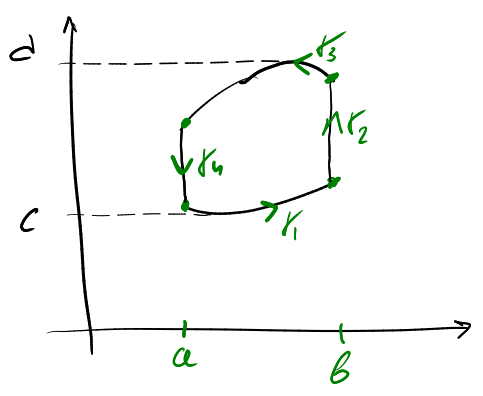
\includegraphics[scale=0.4]{9_1.png}
\end{center}
\(\partial D\) --- состоит из путей \(\gamma_1, \dots, \gamma_4\), где \(\gamma_2, \gamma_4\) --- вертикальные отрезки (возможно вырожденнные ), \(\gamma_1, \gamma_3\) --- гладкие кривые(можно считать, что это графики функций \(\varphi_1(x), \varphi_3(x)\)). Аналогично можно \fixme.
Проверим, что:
\[ - \iint_D \frac{\partial P}{\partial y}\,dx\,dy = \int_{\partial D^+} P\,dx + Q\,dy \]
Левая часть:
\[ - \int_a^b dx \int_{\varphi_1(x)}^{\varphi_3(x)} \frac{\partial P}{\partial y} dy = - \int_a^b P(x, \varphi_3(x)) - P(x, \varphi_1(x)) \,dx \]
Правая часть:
\[ \int_{\gamma_1} + \underbrace{\int_{\gamma_2}}_0 + \int_{\gamma_3} + \underbrace{\int{\gamma_4}}_0 =  \]
\[ = \int_a^b P(x, \varphi_1(x))\,dx - \int_a^b P(x, \varphi_3(x))\, dx \]
\end{proof}
\begin{remark}
Теорема верна для любой области \(D\) с кусочно гладкой границей, которую можно разрезать на криволинейные 4-x угольнинки
\begin{center}
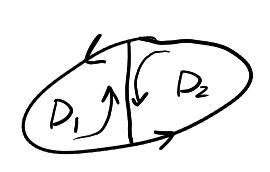
\includegraphics[scale=0.4]{9_2.png}
\end{center}
\[ \int_{\partial D^+} = \int_{\partial D_1^+} + \int_{\partial D_2^+} \fixme \]
\end{remark}
\begin{theorem}[Формула Стокса]
\-
\begin{itemize}
\item \(\Omega\) --- простое гладкое двумерное многообразие в \(\R^3\) (двустороннее)
\item \(n_0\) --- сторона \(\Omega\)
\item \(\partial \Omega\) --- кусочно гладкая кривая
\item \(\partial \Omega^+\) --- ориентированная кривая с согласованной ориентацией.
\item \((P, Q, R)\) --- гладкое векторное поле в окрестности \(\Omega\)
\end{itemize}
\uline{Тогда} \[ \int_{\parial \Omega^+} P\,dx + Q\,dy + R\,dz = \iint_\Omega \left(\frac{\partial R}{\partial y} - \frac{\partial Q}{\partial z}\right)\,dy\,dz + \left(\frac{\partial P}{\partial z} - \frac{\partial R}{\partial x}\right)\,dz\,dx + \left(\frac{\partial Q}{\partial x} - \frac{\partial P}{\partial y}\right)\,dx\,dy \]
\end{theorem}
\begin{proof}
Ограничимся случаем \(\Omega \in C^2\). Достаточно?:
\[ \int_{\partial \Omega^+} P\,dx = \iint_\Omega\frac{\partial P}{\partial z}\,dz\,dx  - \frac{\partial P}{\partial y}\,dx\,dy \]
\[ \Phi = (x(u, v), y(u, v), z(u, v)) \]
\begin{center}
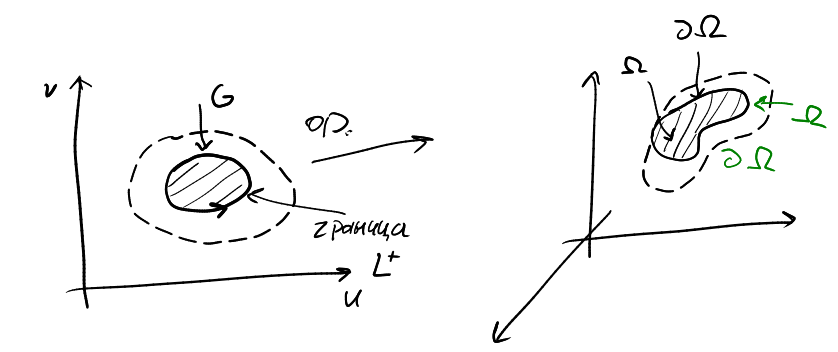
\includegraphics[scale=0.5]{9_3.png}
\end{center}
\color{blue}
\(dx\,dy = - dy\,dx\), \(dx\,dx = 0\)
\[ dP\,dx + dQ\,dy + dR\,dz = (P'_x\,dx + P'_y\,dy + P'_z\,dz)\,dx + \dots \]

\color{black}
\[ \int_{\partial \Omega^+} P\,dx = \int_{L^+} P\cdot (\frac{\partial x}{\partial u}\,du + \frac{\partial x}{\partial v}\,dv) \addtag\label{9_2} \]
\color{blue}
Параметризируем: \(\gamma: [a, b] \to \R^2\), \(\gamma = (u(t), v(t))\) --- параметризируем \(L^+\)
\[ \int_{\partial \Omega^+} P\,dx = \int_a^b P(\frac{\partial dx}{\partial u}u' + \frac{\partial x}{\partial v}v')dt \addtag\label{9_1}\]
\(\Phi \circ \gamma\) --- парметризируем \(\partial \Omega^+\), \((\Phi \circ \gamma)' = \Phi' \cdot \gamma'\)
\[ \ref{9_1} = \int_a^b P\cdot\frac{\partial x}{\partial u}\,du + P \cdot \frac{\partial x}{\partial v}\,dv \]
\color{black}
\[ \ref{9_2} = \iint_G \frac{\partial}{\partial u}\left(P\frac{\partial x}{\partial b}\right) - \frac{\partial}{\partial v} \left(P \frac{\partial x}{\partial u}\right)\,du\,dv = \]
\[ = \iint_G (P'_x\cdot x'_u + P'_y\cdot y'_u + P'_z\cdot z'_u)x'_v + p\cdot x''_{uv} - (P'_x\cdot x'_v + P'_y\cdot y'_v + P'_z\cdot z'_v)x'_u - P\cdot x''_{uv} \,du\,dv = \]
\[ = \iint_G \frac{\partial P}{\partial z} (z'_ux'_v - z'_vx'_u) - \frac{\partial P}{\partial y}(x'_uy'_v - x'_vy'_u) = \iint_G \frac{\partial P}{\partial z}\,dz\,dx - \frac{\partial P}{\partial x}\,dx\,dy\]
\end{proof}

\begin{itemize}
\item \(L^p(X, \mu)\), \(1 \le p \le +\infty\)
\end{itemize}
\[ \left(\int_X |f|^p\,dx\right)^{\frac{1}{p}}\text{ --- сходится} \]
\begin{itemize}
\item \(p = \infty:\ \esssup |f| < +\infty\)
\end{itemize}
\[ \Vert fg \Vert_1 \le \Vert f \Vert_p \cdot \Vert g \Vert_q\]
\begin{theorem}
\-
\begin{itemize}
\item \(\mu E < +\infty\), \(1 \le s < r \le +\infty\)
\end{itemize}
\uline{Тогда}
\begin{enumerate}
\item \(L^r(E, \mu) \subset L^s(E, \mu)\)
\item \(\Vert f \Vert_s \le \muE^{\frac{1}{s} - \frac{1}{r}}\cdot \Vert f \Vert_r\)
\end{enumerate}
\end{theorem}
\begin{proof}
\-
\begin{enumerate}
\item Следует из 2)
\item \begin{description}
\item[{\(r = \infty\)}] \[\left(\int |f|^s\,d\mu\right)^{\frac{1}{s}} \le \esssup |f| \cdot \mu E^{\frac{1}{s}}\]
\item[{\(r < +\infty\)}] \(p := \frac{r}{s}\), \(q = \frac{r}{r - s}\)
\[ \Vert f \Vert_s^s = \int_E |f|^s \,d\mu = \int_E |f|^s\cdot 1 \, d\mu \le \left(\int_E |f|^{s \cdot \frac{r}{s}}\,d\mu\right)^{\frac{s}{r}} \cdot \left(\int_E 1^{\frac{r}{r - s}}\,d\mu\right)^{\frac{r - s}{r}} \le \]
\[ \le \Vert f \Vert_r^s \mu E^{1 - \frac{s}{r}} \]
\end{description}
\end{enumerate}
\end{proof}
\begin{corollary}
\-
\begin{itemize}
\item \(\mu E < +\infty\)
\item \(1 \le s < r \le +\infty\)
\item \(f_n \xrightarrow[L^r]{} f\)
\end{itemize}
\uline{Тогда} \(f_n \xrightarrow[L^s]{} f\)
\end{corollary}
\begin{proof}
\[ \Vert f_n - f \Vert_s \le \mu E^{\frac{1}{r} - \frac{1}{r}} \cdot \Vert f_n - f \Vert_r \to 0 \]
\end{proof}
\begin{theorem}[о сходимости в \(L^p\) и по мере]
\-
\begin{itemize}
\item \(1 \le p < +\infty\)
\item \(f_n \in L^p(X, \mu)\)
\end{itemize}
\uline{Тогда}
\begin{enumerate}
\item \(f \in L^p\), \(f_n \to f\) в \(L^p\) \(\implies\ f_n \xRightarrow[\mu]{} f\)
\item \(f \xRightarrow[\mu]{} f\) либо \(f_n \to f\), \(|f_n| \le g\), \(g \in L^p\) \\
Тогда \(f \in L^p\) и \(f_n \to f\) в \(L^p\)
\end{enumerate}
\end{theorem}
\begin{proof}
\-
\begin{enumerate}
\item \(X_n(\varepsilon) := X(|f_n - f| \ge \varepsilon)\)
\[ \mu X_n(\varepsilon) = \int_{X_n(\varepsilon)} 1 d\mu \le \frac{1}{\varepsilon^p} \int_{X_n(\varepsilon)}|f_n - f|^p\,d\mu\le \frac{1}{\varepsilon^p} \Vert f_n - f \Vert_p^p \to 0 \]
\item \(f_n \Rightarrow f\), \(\exists n_k\ f_{n_k} \to f\) почти везде \(\implies\ |f| \le g\) почти везде \\
\(|f_n - f|^p \le (2g)^p\) --- суммируема (так как \(g \in L^p\)) \\
\(\Vert f_n - f \Vert_p^p \todo\)
\end{enumerate}
\end{proof}
\color{blue}
\begin{itemize}
\item Фундаментальная последовательность: \\
\(\forall \varepsilon > 0\ \exists N\ \forall k, n > N\quad \Vert f_n - f_k \Vert < \varepsilon\), т.е. \(\Vert f_n - f_k \Vert \xrightarrow[n,k\to+\infty]{} 0\)
\item \(f_n \to f\) \implies \(f_n\) --- фундаментальная \(\Vert f_n - f_k \Vert \le \underbrace{\Vert f_n - f \Vert}_{\to 0} + \underbrace{\Vert f - f_k \Vert}_{\to 0}\)
\item \(C(k)\) --- пространство непрерывных функций на компакте \(K\) \\
\(\Vert f \Vert = \max_K |f|\), утверждение: \(C(K)\) --- полное
\end{itemize}
\color{black}
\begin{task}
\(L^{\infty}(X, \mu)\) --- полное
\end{task}
\begin{theorem}
\-
\begin{itemize}
\item \(L^p(X, \mu)\) --- полное
\item \(1 \le p < +\infty\)
\end{itemize}
\end{theorem}
\begin{proof}
\(f_n\) --- фундаментальная
\[ \varepsilon = \frac{1}{2}\ \exists N_1\ \forall n_1, k > N\quad \Vert f_{n_1} - f_k \Vert_p < \frac{1}{2} \]
Возьмем один такой \(n_1\) и зафиксируем:
\[ \varepsilon = \frac{1}{4}\ \exists N_2 > n_1\ \forall n_2, k > N_2\quad \Vert f_{n_2} - f_k \Vert_p < \frac{1}{4} \]
Повторим это действие. Получим последовательность \((n_k)\):
\[ \sum_k \Vert f_{n_{k + 1}} - f_{n_k} \Vert_p < 1 \]
Рассмотрим ряд:
\[S(x) = \sum_k |f_{n_{k + 1}}(x) - f_{n_k}(x) |\quad S(x) \in [0, +\infty]\]
\(S_N\) --- частичные суммы ряда \(S\)
\[ \Vert S_N \Vert_p \le \sum_{k = 1}^N \Vert f_{n_{k + 1}} - f_{n_k} \Vert_p \< 1 \]
, т.е. \(\int_X S_N^p < 1\), по теореме Фату: \(\int_X S^p\,d\mu < 1\), т.е. \(S^p\) --- суммируема \implies \(S\) --- почти везде конечна 
\[ f(x) = f_{n_1}(x) + \sum_{k = 1}^{+\infty} (f_{n_{k + 1}}(x) - f_{n_k}(x)) \]
--- его частичные суммы --- это \(f_{n_{N + 1}}(x)\), т.е. схоимость этого ряда почти везде означает, что \(f_{n_k} \to f\) почти везде. Проверим, что \(\Vert f_n - f \Vert_p \to 0\)
\[ \forall \varepsilon > 0\ \exists N\ \forall m,n > N\quad \Vert f_n - f_m \Vert_p < \varepsilon \]
Берем \(m = n_k > N\)
\[ \Vert f_n - f_{n_k} \Vert_p^p = \int_X |f_n - f_{n_k} | ^p\,d\mu < \varepsilon^p \]
это выполняется при всех больших \(k\). По теореме Фату:
\[ \int_X | f_n - f |^p d\mu < \varepsilon^p \]
, т.е. \(\Vert f_n - f \Vert < \varepsilon\)
\end{proof}
\begin{definition}
\(Y\) --- метрическое пространство, \(A \subset Y\), \(A\) --- (всюду) плотно в \(Y\)
\[ \forall y in Y\ \forall U(y)\ \exists a \in A:\ a\in U(y) \]
\end{definition}
\begin{examp}
\(\mathbb{Q}\) плотно в \(\R\)
\end{examp}
\begin{lemma}
\-
\begin{itemize}
\item \((X, \A, \mu)\)
\item \(1 \le p \le +\infty\)
\end{itemize}
Множество ступенчатых функций (из \(L^p\)) плотно в \(L^p\)
\end{lemma}
\begin{remark}
\(\varphi \in L^p\) --- ступенчатая \implies \(\muX(\varphi \neq 0) < +\infty\)
\end{remark}
\begin{proof}
\-
\begin{description}
\item[{\(p = \infty\)}] \(f \in L^\infty\), изменив \(f\) на множестве \(C\) меры \(0\), считаем, что \(|f| \le \Vert f \Vert_\infty\). Тогда существуют ступенчатые \(0\le\varphi_n \rightrightarrows f^+\), \(0 \le \psi_n \rightrightarrows f^-\). Тогда сколько угодно близко к \(f\) можно найти ступенчатую фкнцию вида \(\varphi_n + \psi_n\)
\item[{\(p < +\infty\)}] Пусть \(f \ge 0\). \(\exists \varphi_n \ge 0\) --- ступенчатая: \(\varphi_n \uparrow f\)
\[ \Vert \varphi_n - f \Vert^p_p = \int_X | \varphi_n - f |^p \to 0 \]
, по теореме Лебега. \(f\) --- любого знака: берем \(f^+, f^-, \dots\)
\end{description}
\end{proof}
\begin{definition}
\(f: \R^m \to \R\) --- \textbf{финитная}, если \(\exists B(0, r): f\equiv 0\) вне \(B(0, r)\). \\
\(C_0(\R^m)\) --- непрерывные финитные функции. \(\forall p \ge 1\ C_0(\R^m) \subset L^p(\R^m, \lambda_m)\)
\end{definition}
\begin{definition}
Топологическое пространство \(X\) --- \textbf{нормальное}, если
\begin{enumerate}
\item Точки \(X\) --- замкнутые множества
\item \(\forall F_1, F_2 \subset X\) --- замкнутые, \(\exists U(F_1), U(F_2)\) --- открытые и \(U(F_1)\cap U(F_2) = \emptyset\)
\end{enumerate}
\end{definition}
\begin{task}
\(R^m\) --- нормальное
\end{task}
\end{document}
